\documentclass[border=10pt]{standalone}
\usepackage{pgfplots}
\pgfplotsset{compat=1.18}
\begin{document}
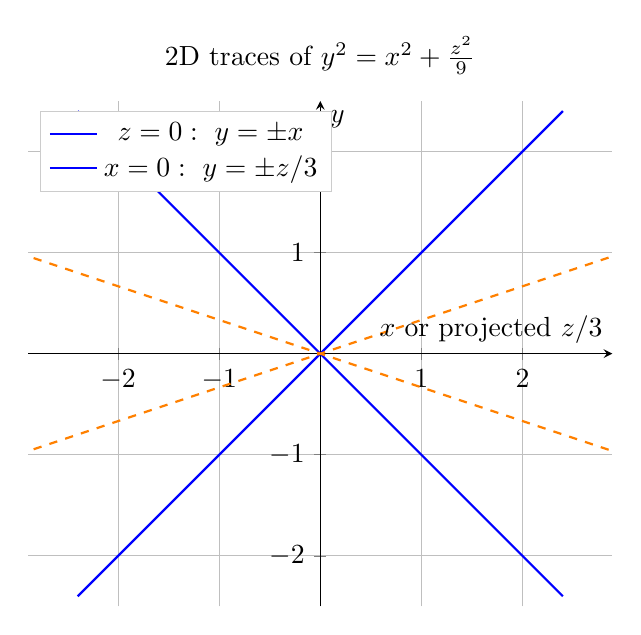
\begin{tikzpicture}
\begin{axis}[
  width=9cm,
  height=8cm,
  axis lines=center,
  xlabel={$x$ or projected $z/3$},
  ylabel={$y$},
  xmin=-2.5, xmax=2.5,
  ymin=-2.5, ymax=2.5,
  grid=major,
  axis equal,
  title={2D traces of $y^2=x^2+\frac{z^2}{9}$},
  legend style={at={(0.02,0.98)}, anchor=north west, draw=black!20}
]
\addplot[blue, thick, domain=-2.4:2.4, samples=100] {x};
\addplot[blue, thick, domain=-2.4:2.4, samples=100] {-x};
\addlegendentry{$z=0:\ y=\pm x$};
\addplot[orange, thick, dashed, domain=-7.2:7.2, samples=100] {x/3};
\addplot[orange, thick, dashed, domain=-7.2:7.2, samples=100] {-x/3};
\addlegendentry{$x=0:\ y=\pm z/3$};
\end{axis}
\end{tikzpicture}
\end{document}
